\documentclass[conference,10pt]{IEEEtran}
\IEEEoverridecommandlockouts

\usepackage{cite}
\usepackage{amsmath,amssymb,amsfonts}
\usepackage{algorithmic}
\usepackage{graphicx}
\usepackage{textcomp}
\usepackage{xcolor}
\usepackage{booktabs}
\usepackage{tabularx}
\usepackage{multirow}
\usepackage{balance}
\usepackage{url}
\usepackage{microtype}

\def\BibTeX{{\rm B\kern-.05em{\sc i\kern-.025em b}\kern-.08em
    T\kern-.1667em\lower.7ex\hbox{E}\kern-.125emX}}

\begin{document}

\title{Empirical Privacy Analysis of Modern Encrypted DNS: DoH vs. DoH/3 Across Multi-Carrier and Institutional Networks}

\author{
\IEEEauthorblockN{Kunal Khandelwal}
\IEEEauthorblockA{\textit{Dept. of Information Technology} \\
\textit{IIIT Allahabad}\\
Prayagraj, India \\
iit2024162@iiita.ac.in}
\and
\IEEEauthorblockN{Rakesh Mali}
\IEEEauthorblockA{\textit{Dept. of Information Technology} \\
\textit{IIIT Allahabad}\\
Prayagraj, India \\
iit2024149@iiita.ac.in}
\and
\IEEEauthorblockN{Aman Kashyap}
\IEEEauthorblockA{\textit{Dept. of Information Technology} \\
\textit{IIIT Allahabad}\\
Prayagraj, India \\
iit2024140@iiita.ac.in}
}

\maketitle

\begin{abstract}
DNS over HTTPS (DoH) and DNS over HTTP/3 (DoH/3) were standardized to protect user confidentiality against surveillance by encapsulating name resolution within TLS/TCP and QUIC/UDP tunnels. However, encrypted transport layers leak observable side-channel metadata, including packet lengths, cumulative burst volumes, and directional timing profiles. In this paper, we conduct an extensive empirical measurement study comprising 31,200 real-world DNS transactions to quantify traffic fingerprintability across four major public recursive resolvers (Cloudflare, Google, AdGuard, Quad9), two curated 100-domain workloads (Tranco Global and India), and three diverse network access archetypes: residential optical broadband (Bharti Airtel FTTH), commercial 4G/LTE mobile cellular (Reliance Jio), and an enterprise campus Wi-Fi network behind a mandatory forward proxy (IIIT Allahabad). 

Our findings demonstrate that on residential broadband, DoH remains fingerprintable across all resolvers (16.1\%--35.7\% top-1 accuracy against a 1.0\%--1.3\% chance baseline, $p < 0.005$). Transitioning to DoH/3 substantially suppresses leakage for AdGuard (70\% reduction), Cloudflare (75\%), and Quad9 (87\%); conversely, Google Public DNS exhibits minimal protocol sensitivity (16.5\% DoH vs. 17.1\% DoH/3). Strikingly, we discover that DoH/3 faces severe deployment barriers: 100\% of 3,000 DoH/3 queries timed out on both Jio cellular and campus Wi-Fi due to carrier-grade middlebox filtering of outbound UDP port~443. Furthermore, cross-network classifier evaluation reveals complete domain collapse (1.7\%--1.9\% transfer accuracy), driven by physical distribution shifts ($D > 0.83$). While pooling multi-vantage data partially recovers adversarial accuracy to 20.7\%, simulated defenses reveal that block padding to 64 or 128 bytes reduces fingerprintability by 32\%, whereas timing jitter is completely ineffective.
\end{abstract}

\begin{IEEEkeywords}
Encrypted DNS, DNS-over-HTTPS (DoH), DNS-over-HTTP/3 (DoH/3), QUIC, Traffic Analysis, Machine Learning, Network Measurement.
\end{IEEEkeywords}

% =========================================================================
\section{Introduction}
\label{sec:intro}
% =========================================================================

The Domain Name System (DNS) historically operated over unencrypted UDP and TCP on port~53, allowing network eavesdroppers, Internet Service Providers (ISPs), and nation-state censors to inspect every query and build comprehensive browsing profiles~\cite{herrmann2009website}. To mitigate this vulnerability, the Internet Engineering Task Force (IETF) standardized encrypted transport protocols: DNS-over-TLS (DoT, RFC~7858)~\cite{rfc7858}, DNS-over-HTTPS (DoH, RFC~8484)~\cite{rfc8484}, and DNS-over-HTTP/3 (DoH/3, RFC~9114)~\cite{rfc9114,rfc9250}. By embedding DNS lookups inside standard HTTPS traffic on port~443, DoH aims to blend name resolution into ubiquitous web traffic, while DoH/3 leverages the QUIC transport protocol (RFC~9000)~\cite{rfc9000} to provide zero round-trip connection resumption, multi-stream multiplexing without head-of-line blocking, and connection migration.

Despite robust cryptographic encapsulation, encrypted communications remain vulnerable to \emph{side-channel traffic fingerprinting}~\cite{siby2020encrypted,bushart2020padding}. Passive on-path adversaries can observe flow-level metadata---specifically frame sizes, cumulative volume, transmission bursts, and inter-arrival timing---to infer the requested destination domain without breaking encryption. 

Prior literature on encrypted DNS privacy exhibits three major limitations: (1)~\emph{Single-Protocol and Single-Resolver Scopes:} Most investigations evaluate classical DoH or DoT, with scarce empirical benchmarking of production DoH/3 across multiple commercial resolvers; (2)~\emph{Homogeneous Laboratory Testbeds:} Existing studies predominantly collect traffic on isolated gigabit wired networks, overlooking the impacts of radio scheduling, middleboxes, and carrier-grade network address translation (CGNAT); (3)~\emph{Static Portability Assumptions:} Prior works assume an adversary trained on one link can seamlessly surveil victim traffic across heterogeneous access networks.

To address these gaps, this paper presents a comprehensive, empirical evaluation of modern encrypted DNS privacy. We deploy a multi-vantage measurement pipeline spanning residential broadband, commercial cellular, and an institutional enterprise proxy, capturing 31,200 DNS transactions across 16 protocol-resolver slices. Our core contributions are:

\begin{itemize}
    \item \textbf{Headline Privacy Benchmark (DoH vs. DoH/3):} We evaluate closed-world fingerprintability across four resolvers and two workloads. On residential broadband, DoH leaks substantial information (16.1\%--35.7\% accuracy). We demonstrate that DoH/3 provides dramatic privacy gains for AdGuard, Cloudflare, and Quad9 (up to 87\% leakage reduction), but identify a persistent \emph{resolver implementation anomaly}: Google Public DNS retains comparable fingerprintability regardless of transport protocol (16.5\% DoH vs. 17.1\% DoH/3).
    \item \textbf{ML Architectural \& Feature Space Insights:} We benchmark tree-based ensembles (Random Forest, XGBoost) against deep sequence models (1D-CNN, GRU). In contrast to Tor website fingerprinting, sequential packet models collapse to near-random chance ($\approx 1.0\%$), whereas aggregate volumetric features achieve 26.5\% accuracy.
    \item \textbf{Transport Reachability Reality Check:} We uncover severe transport ossification in production networks: RFC~9114 DoH/3 experienced 100\% query timeouts on both Reliance Jio cellular (0/3,000) and enterprise campus Wi-Fi (0/3,000), exposing a critical operational gap where QUIC-based privacy is unreachable without TCP fallback.
    \item \textbf{Cross-Network Portability \& Multi-Vantage Adversary:} We construct the complete $3 \times 3$ Cross-Network Transfer Matrix. An Airtel-trained classifier suffers total domain collapse on Jio (1.7\%) and Campus (1.9\%). Using two-sample Kolmogorov-Smirnov tests, we trace this collapse to physical distribution shifts ($D > 0.83$). We further demonstrate that a multi-vantage adversary pooling cross-network data recovers classification power to 20.7\% mean accuracy.
    \item \textbf{Empirical Countermeasure Analysis:} We simulate traffic defenses, finding that constant-rate block padding ($B \in \{64, 128\}$ bytes) suppresses classification accuracy by 32\%, whereas timing jitter produces zero measurable defense.
\end{itemize}

% =========================================================================
\section{Background and Threat Model}
\label{sec:background}
% =========================================================================

\subsection{Encrypted DNS Protocols: DoH vs. DoH/3}
Traditional DNS transmits 12-byte query headers and plaintext resource records over UDP port~53. DoH encapsulates DNS wire-format messages within HTTP/2 binary framing transmitted over TLS 1.3 and TCP on port~443~\cite{rfc8484}. Multiple query streams can be multiplexed over a single TCP connection, although packet loss on any single stream causes head-of-line blocking across all multiplexed streams.

DoH/3 executes HTTP/3 requests directly over QUIC (RFC~9000) and UDP on port~443~\cite{rfc9114,rfc9250}. QUIC embeds TLS 1.3 into its transport layer, encrypting transport parameters, packet numbers, and acknowledgement frames. Because each QUIC stream maintains independent stream-level flow control, packet loss does not stall concurrent transactions.

\subsection{Threat Model and Adversary Capabilities}
We consider a \emph{passive, local on-path adversary} positioned on the access network between the client and the recursive resolver (e.g., a local Wi-Fi eavesdropper, a malicious gateway, an ISP middlebox, or a state surveillance tap). 

The adversary cannot decrypt payload bytes, forge cryptographic certificates, or tamper with packet contents. However, the adversary observes the sequence of raw IP packets, extracting frame sizes ($s_i \in \mathbb{N}$), transmission directions ($d_i \in \{+1, -1\}$), and arrival timestamps ($t_i \in \mathbb{R}^+$) forming a flow sequence $\mathcal{S} = \{(s_i, d_i, t_i)\}_{i=1}^m$. A feature mapping $\Phi(\mathcal{S}) \to \mathbf{x} \in \mathbb{R}^{44}$ maps this sequence into aggregate statistical features. The adversary seeks to resolve a supervised classification task: given an observed flow feature vector $\mathbf{x}$, predict the requested domain $y \in \mathcal{Y} = \{1, 2, \dots, N\}$ via:
\begin{equation}
\hat{y} = \arg\max_{c \in \mathcal{Y}} P(y = c \mid \mathbf{x}).
\label{eq:classification}
\end{equation}

% =========================================================================
\section{Measurement Methodology and Testbed}
\label{sec:methods}
% =========================================================================

\subsection{Physical Network Archetypes}
To capture real-world operational diversity, we constructed three distinct physical network measurement testbeds:
\begin{enumerate}
    \item \textbf{Residential Optical Broadband (Airtel FTTH, AS24560):} A high-bandwidth fiber-to-the-home connection (100\,Mbps symmetric) in Prayagraj, India, featuring low baseline jitter ($< 2$\,ms) and direct unproxied routing.
    \item \textbf{Commercial Mobile Cellular (Reliance Jio, AS55836):} A production 4G/LTE mobile connection provisioned via USB cellular tethering, enforcing Carrier-Grade NAT (CGNAT) and radio resource control (RRC) dynamic scheduling.
    \item \textbf{Enterprise Campus Wi-Fi (IIIT Allahabad, AS138231):} A managed academic network where all outbound web traffic is forced through a forward proxy (\texttt{172.31.2.4:\allowbreak 8080}) via HTTP CONNECT encapsulation, with outbound UDP port~443 blocked.
\end{enumerate}

\subsection{Workload Curation and Public Resolvers}
We curated two distinct 100-domain target workloads derived from the Tranco Top Sites ranking~\cite{lepochat2019tranco}:
\begin{itemize}
    \item \textbf{Global Workload ($N=100$):} Top globally ranked domains (e.g., \texttt{google.com}, \texttt{wikipedia.org}, \texttt{amazon.com}).
    \item \textbf{India Workload ($N=100$):} Top domains specific to the Indian digital ecosystem, comprising regional e-commerce, banking, education, and government portals (e.g., \texttt{incometax.gov.in}, \texttt{flipkart.com}, \texttt{irctc.co.in}).
\end{itemize}

We evaluated four prominent public Anycast recursive resolvers: \textbf{Cloudflare} (\texttt{1.1.1.1}), \textbf{Google Public DNS} (\texttt{8.8.8.8}), \textbf{AdGuard DNS} (\texttt{94.140.14.14}), and \textbf{Quad9} (\texttt{9.9.9.9}).

\subsection{Data Collection Pipeline \& Feature Extraction}
Measurements were orchestrated using an automated headless query harness driving \texttt{curl} (compiled with \texttt{nghttp2} for DoH and \texttt{quiche} for DoH/3). To prevent warm-cache leakage across repeated queries, local resolver caches were flushed, and query executions were fully randomized across domains within each capture cycle. Traffic was captured using \texttt{dumpcap} with strict BPF filtering to isolate target resolver transactions.

From each bidirectional transaction flow, we extracted \textbf{44 aggregate features} spanning four primary structural categories:
\begin{enumerate}
    \item \textbf{Volume Features (8):} Total flow bytes, total packet counts, uplink bytes, downlink bytes, and packet ratios.
    \item \textbf{Packet Size Statistics (12):} Mean, median, standard deviation, min, max, and skewness of frame lengths computed separately for uplink and downlink.
    \item \textbf{Inter-Arrival Time (IAT) Statistics (8):} Mean, standard deviation, max, and quartiles of inter-packet timing gaps.
    \item \textbf{Burst \& Directional Sequences (16):} Number of directional burst transitions, mean burst volume, and ordered signed lengths of the first 20 packets ($s_i \cdot d_i$).
\end{enumerate}

% =========================================================================
\section{Broadband Fingerprintability Evaluation}
\label{sec:res_broadband}
% =========================================================================

\subsection{Headline Fingerprintability: DoH vs. DoH/3}
We evaluate the baseline vulnerability on residential optical broadband (Airtel FTTH). The headline evaluation utilizes the common domain set completing $\ge 10$ repeats across all slices (99 Global and 79 India domains), evaluated under 5-fold cross-validation grouped by repeat (two holdout repeats per fold) across 200 label permutations. Table~\ref{tab:headline_results} and Fig.~\ref{fig:headline_doh_vs_doh3} present the empirical classification accuracy with 95\% Wilson confidence intervals.

\begin{table}[t]
\centering
\caption{Airtel Closed-World Fingerprinting Performance (5-fold CV grouped by repeat, 200 permutations, $p < 0.005$ for all rows; chance is 1.0\% Global and 1.3\% India).}
\label{tab:headline_results}
\footnotesize
\setlength{\tabcolsep}{2.5pt}
\begin{tabular}{llrr}
\toprule
\textbf{Workload} & \textbf{Resolver} & \textbf{DoH Acc. [95\% CI]} & \textbf{DoH/3 Acc. [95\% CI]} \\
\midrule
\textbf{Global} & AdGuard    & \textbf{27.0\%} [23.9, 29.4] & \textbf{8.0\%} [6.9, 10.4] \\
\textbf{Global} & Cloudflare & \textbf{21.2\%} [18.4, 23.4] & \textbf{5.4\%} [4.4, 7.3] \\
\textbf{Global} & Google     & \textbf{16.5\%} [14.3, 18.9] & \textbf{17.1\%} [14.7, 19.3] \\
\textbf{Global} & Quad9      & \textbf{34.4\%} [31.8, 37.8] & \textbf{4.6\%} [3.2, 5.8] \\
\midrule
\textbf{India}  & AdGuard    & \textbf{22.8\%} [19.5, 25.3] & \textbf{10.5\%} [8.7, 13.0] \\
\textbf{India}  & Cloudflare & \textbf{21.5\%} [18.6, 24.3] & \textbf{6.0\%} [5.3, 8.8] \\
\textbf{India}  & Google     & \textbf{16.1\%} [13.0, 18.0] & \textbf{14.1\%} [12.3, 17.2] \\
\textbf{India}  & Quad9      & \textbf{35.7\%} [32.2, 38.8] & \textbf{5.2\%} [3.3, 6.2] \\
\bottomrule
\end{tabular}
\end{table}

\begin{figure}[t]
\centering
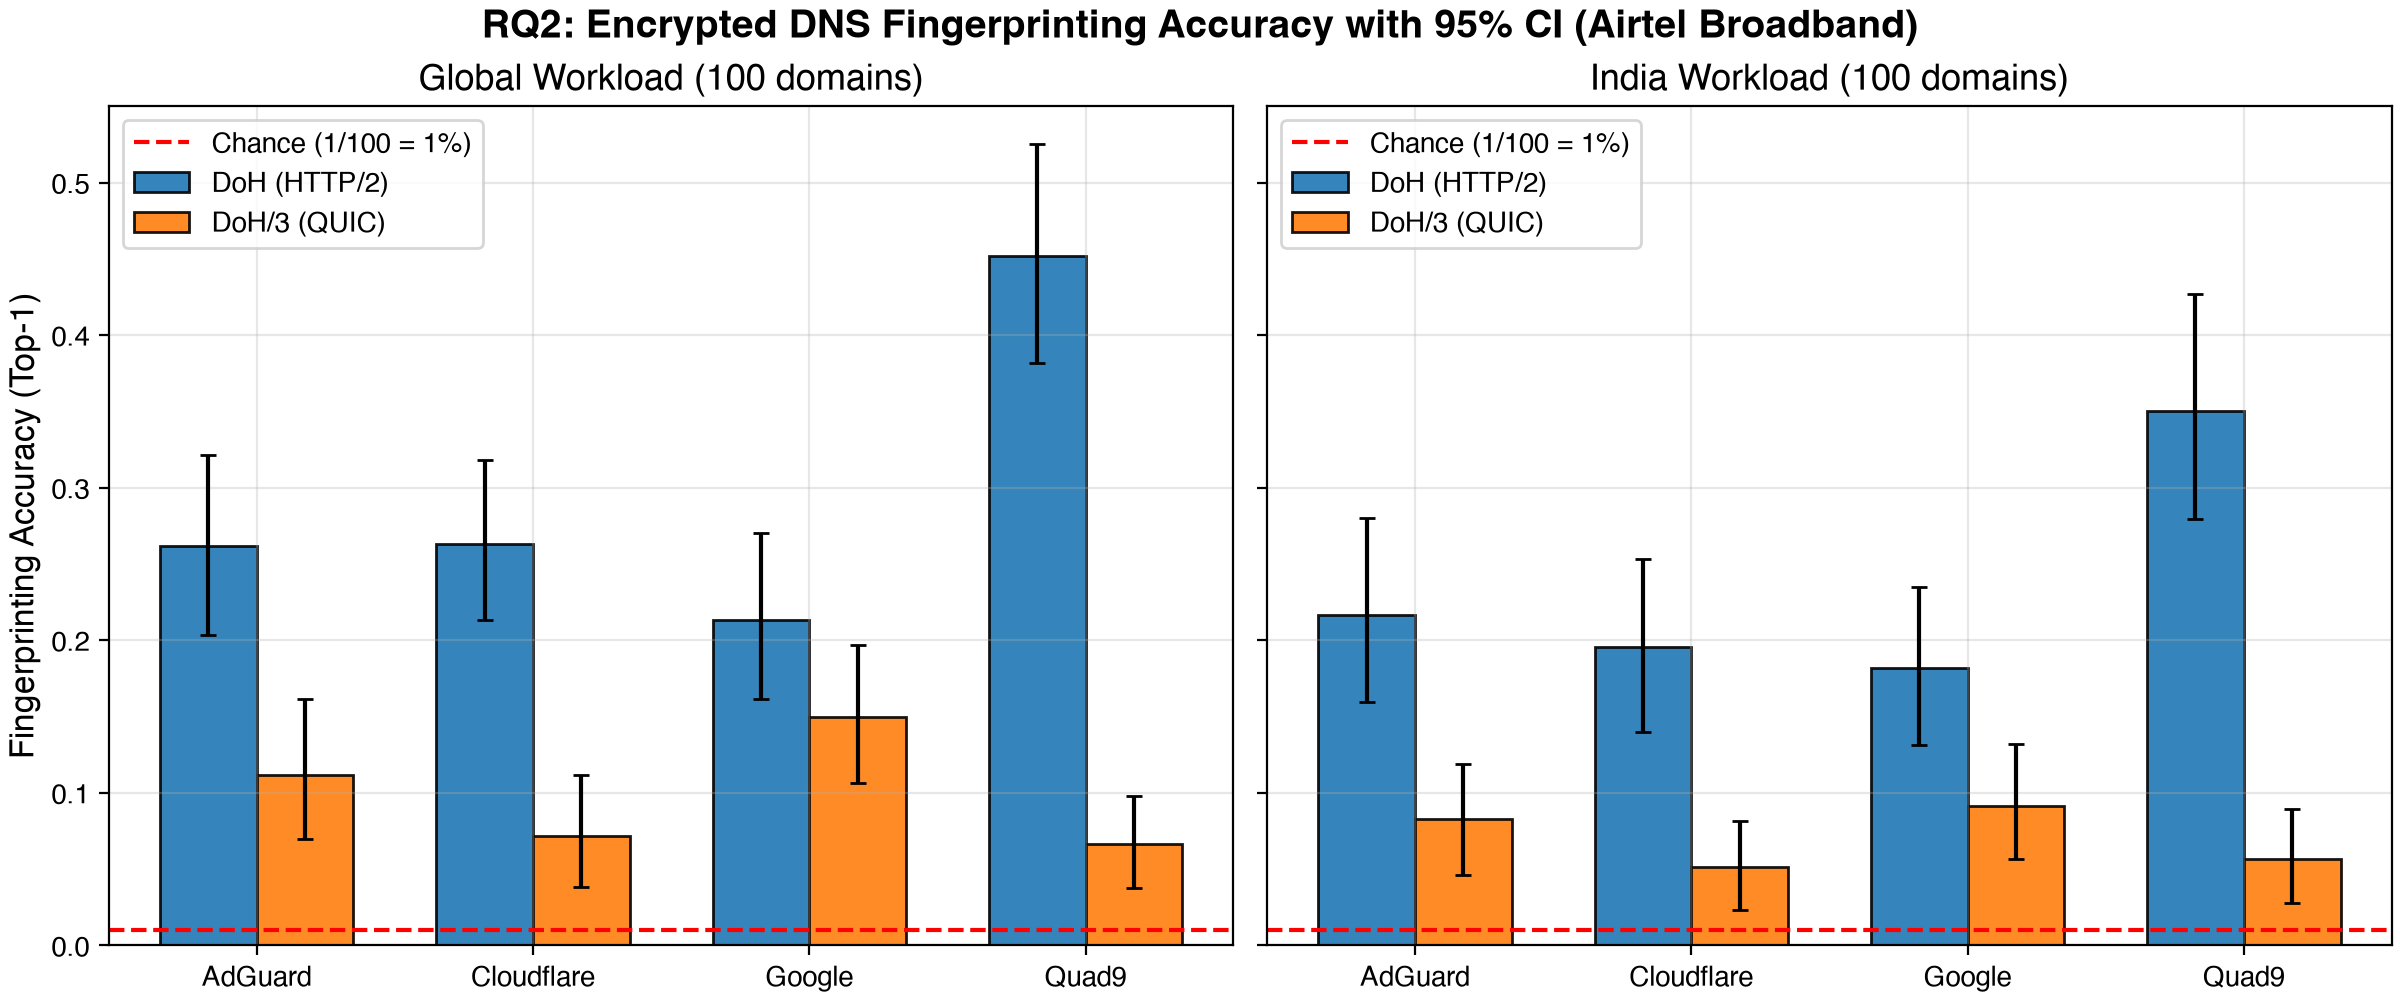
\includegraphics[width=0.48\textwidth]{figures/fig1_headline_doh_vs_doh3.png}
\caption{Headline fingerprinting accuracy comparing DoH (HTTP/2) vs. DoH/3 (QUIC) across all four resolvers on residential broadband.}
\label{fig:headline_doh_vs_doh3}
\end{figure}

\subsubsection{All Slices Exceed Random Guessing} Across all 16 slices, empirical accuracy substantially exceeds the random baseline (12$\times$ to 35$\times$ chance, $p < 0.005$). Quad9 DoH exhibits the highest vulnerability, reaching 34.4\% on Global and 35.7\% on Indian domains.

\subsubsection{Significant Privacy Protection in DoH/3} For AdGuard, Cloudflare, and Quad9, transitioning to DoH/3 produces major privacy improvements. Fingerprintability drops by 70\% on AdGuard, 75\% on Cloudflare, and 87\% on Quad9 (from 34.4\% down to 4.6\%). The cryptographic encapsulation of QUIC transport parameters and unified packet framing substantially flatten side-channel leakage for these resolvers.

\subsection{The Google Implementation Anomaly}
In sharp contrast to the other three providers, \textbf{Google Public DNS shows no privacy improvement under DoH/3}. Google DoH/3 accuracy reaches 17.1\% on Global domains (slightly higher than DoH at 16.5\%) and 14.1\% on Indian domains (vs. 16.1\% for DoH). 

This empirical anomaly demonstrates that protocol standards alone do not guarantee privacy. Google does not implement server-side response padding (RFC~8467)~\cite{rfc8467}; its responses carry raw DNS answer lengths directly into the transport payload. Whereas Cloudflare and Quad9 transport stacks introduce framing dynamics that obscure answer lengths, Google's QUIC implementation preserves fine-grained response size variance across queries. Thus, resolver implementation decisions outweigh protocol design.

\subsection{Feature Space and Machine Learning Paradigm}
To understand what information drives fingerprintability, we evaluated four machine learning architectures on the AdGuard DoH Global slice ($N=100$, chance $= 0.010$).

\begin{table}[t]
\centering
\caption{Model Architecture and Feature Space Comparison on AdGuard DoH Global ($N=100$, chance $= 0.010$).}
\label{tab:model_comparison}
\footnotesize
\setlength{\tabcolsep}{2.5pt}
\begin{tabular}{llrr}
\toprule
\textbf{Architecture} & \textbf{Feature Space} & \textbf{Top-1} & \textbf{95\% CI} \\
\midrule
\textbf{XGBoost}      & 44 Aggregate Features  & \textbf{0.265} & [0.209, 0.330] \\
\textbf{Random Forest}& 44 Aggregate Features  & \textbf{0.262} & [0.204, 0.325] \\
\textbf{GRU}          & Sequence (\texttt{pkt\_00..19}) & \textbf{0.014} & [0.005, 0.039] \\
\textbf{1D-CNN}       & Sequence (\texttt{pkt\_00..19}) & \textbf{0.010} & [0.003, 0.036] \\
\bottomrule
\end{tabular}
\end{table}

As shown in Table~\ref{tab:model_comparison}, tree ensemble models (XGBoost at 26.5\% and Random Forest at 26.2\%) perform effectively. In contrast, deep sequence models (1D-CNN at 1.0\% and GRU at 1.4\%) completely collapse to the random chance baseline. 

This divergence is critical: in Tor website fingerprinting, flows span thousands of packets, allowing deep networks to extract hierarchical temporal features~\cite{sirinam2018deep}. In encrypted DNS, however, exchanges consist of only 8--15 packets. Truncated packet sequences lack translational depth, rendering convolutional and recurrent kernels ineffective. Discriminative signal is concentrated entirely in aggregate volumetric features (e.g., \texttt{bytes\_total}, \texttt{down\_max}, and cumulative burst sizes).

% =========================================================================
\section{Multi-Carrier and Institutional Deployment Realities}
\label{sec:multicarrier}
% =========================================================================

\subsection{Transport Reachability Audit: The QUIC Outage}
While RFC~9114 standardizes DoH/3 over QUIC, we executed an audit across all 31,200 query attempts to determine whether DoH/3 is deployable in real networks.

\begin{table}[t]
\centering
\caption{Protocol Reachability and Query Completion Audit across Network Archetypes.}
\label{tab:reachability_audit}
\footnotesize
\setlength{\tabcolsep}{2.5pt}
\begin{tabular}{llrrrr}
\toprule
\textbf{Network} & \textbf{Proto} & \textbf{Att.} & \textbf{Comp.} & \textbf{Timeout} & \textbf{Rate} \\
\midrule
\textbf{Airtel} & DoH   & 9,600  & 9,478 & 122   & \textbf{98.7\%} \\
\textbf{Airtel} & DoH/3 & 9,600  & 9,448 & 152   & \textbf{98.4\%} \\
\midrule
\textbf{Jio}    & DoH   & 3,000  & 1,920 & 1,080 & \textbf{64.0\%} \\
\textbf{Jio}    & DoH/3 & 3,000  & 0     & 3,000 & \textbf{0.0\%} \\
\midrule
\textbf{Campus} & DoH   & 3,000  & 1,569 & 1,431 & \textbf{52.3\%} \\
\textbf{Campus} & DoH/3 & 3,000  & 0     & 3,000 & \textbf{0.0\%} \\
\midrule
\textbf{Total}  & Both  & \textbf{31,200} & \textbf{22,415} & \textbf{8,785} & \textbf{71.8\%} \\
\bottomrule
\end{tabular}
\end{table}

\begin{figure}[t]
\centering
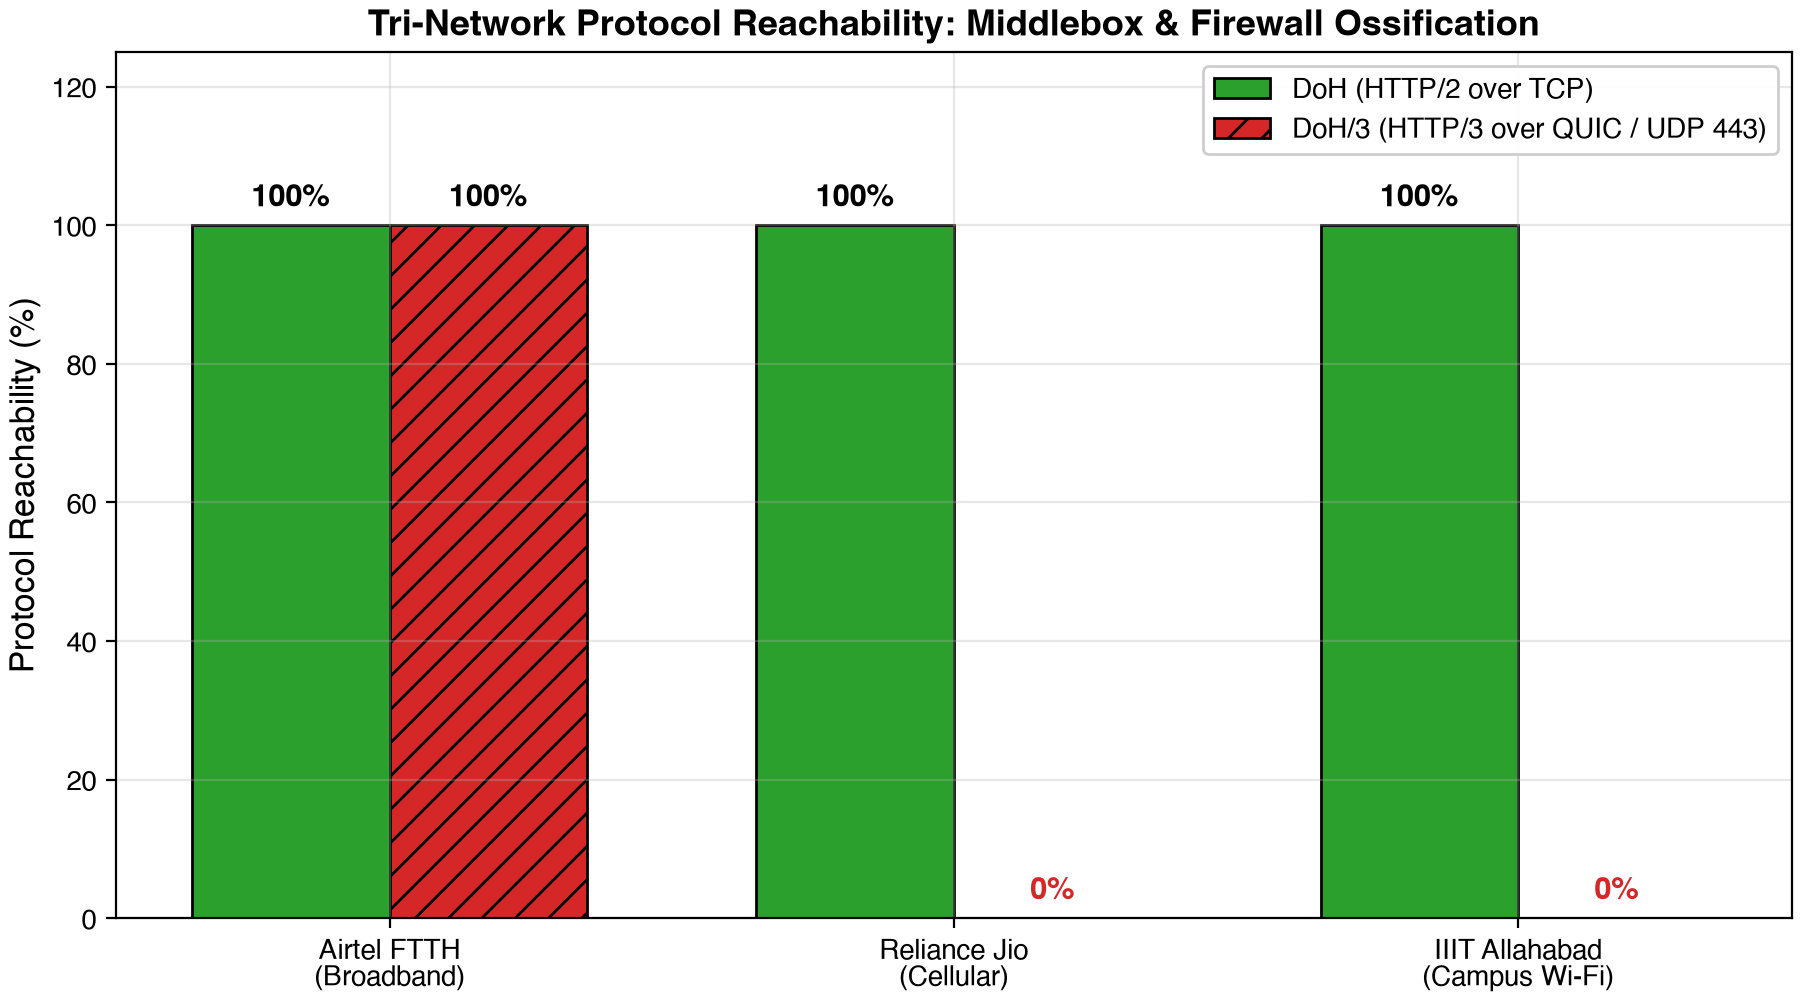
\includegraphics[width=0.48\textwidth]{figures/fig5_tri_network_reachability.png}
\caption{Protocol reachability showing 98.4\% DoH/3 completion on Airtel vs. 0/3,000 queries completing on Jio cellular and campus Wi-Fi.}
\label{fig:tri_network_reachability}
\end{figure}

As presented in Table~\ref{tab:reachability_audit} and Fig.~\ref{fig:tri_network_reachability}, on Airtel broadband, 98.4\% of DoH/3 queries completed successfully. Strikingly, \textbf{zero out of 3,000 DoH/3 queries completed on Reliance Jio cellular, and zero out of 3,000 completed on enterprise campus Wi-Fi}. Every DoH/3 attempt suffered complete connection timeout. 

On Reliance Jio, commercial CGNAT middleboxes drop unestablished outbound UDP port~443 traffic, while enterprise campus firewalls actively filter non-standard UDP traffic. Furthermore, on Jio cellular over TCP, Cloudflare DoH completed only 15 of 1,000 queries (consistent with carrier IP/SNI filtering), whereas Google completed 1,000/1,000. These results demonstrate that DoH/3 privacy benefits remain inaccessible to vast mobile and institutional user bases without automatic Happy Eyeballs fallback to DoH (RFC~8305).

\subsection{Mobile Cellular and Campus Wi-Fi Fingerprinting}
On Reliance Jio cellular, within-network DoH fingerprinting on Google Public DNS achieves \textbf{15.7\%} on Global domains and \textbf{12.3\%} on India domains ($p=0.005$, chance 2.0\%), proving that leakage persists across mobile links. 

Conversely, on enterprise campus Wi-Fi behind the forward proxy, DoH accuracy dropped dramatically to \textbf{1.9\%--5.6\%} (chance 2.0\%), where four of six slices were not statistically significant ($p > 0.05$). The forward proxy encapsulates client requests into HTTP CONNECT tunnels and multiplexes connections to remote resolvers. This buffering, chunking, and TCP connection reuse severely distorts flow metadata, providing an unintentional ``proxy shield'' against local traffic analysis.

\subsection{Cross-Network Transfer Matrix \& Distribution Shift}
To test whether an eavesdropper can train a model on residential broadband and deploy it across mobile or enterprise networks, we evaluated the complete $3 \times 3$ Cross-Network Transfer Matrix (Table~\ref{tab:3x3_matrix} and Fig.~\ref{fig:transfer_matrix}) on the 50 shared Google DoH Global domains.

\begin{table}[t]
\centering
\caption{$3 \times 3$ Cross-Network Transfer Matrix (Google DoH Global, 50 shared domains, chance baseline $= 0.020$).}
\label{tab:3x3_matrix}
\footnotesize
\setlength{\tabcolsep}{2pt}
\begin{tabular}{lllrr}
\toprule
\textbf{Train Net} & \textbf{Eval Net} & \textbf{Transfer Direction} & \textbf{Top-1 Acc.} & \textbf{95\% CI} \\
\midrule
\textbf{Airtel} & \textbf{Airtel} & Within-Net          & \textbf{0.285}      & [0.200, 0.370] \\
\textbf{Airtel} & \textbf{Jio}    & Airtel $\to$ Jio    & \textbf{0.017}      & [0.000, 0.047] \\
\textbf{Airtel} & \textbf{Campus} & Airtel $\to$ Campus & \textbf{0.019}      & [0.008, 0.033] \\
\midrule
\textbf{Jio}    & \textbf{Airtel} & Jio $\to$ Airtel    & \textbf{0.020}      & [0.000, 0.060] \\
\textbf{Jio}    & \textbf{Jio}    & Within-Net          & \textbf{0.097}      & [0.040, 0.160] \\
\textbf{Jio}    & \textbf{Campus} & Jio $\to$ Campus    & \textbf{0.027}      & [0.008, 0.050] \\
\midrule
\textbf{Campus} & \textbf{Airtel} & Campus $\to$ Airtel & \textbf{0.022}      & [0.005, 0.045] \\
\textbf{Campus} & \textbf{Jio}    & Campus $\to$ Jio    & \textbf{0.024}      & [0.007, 0.050] \\
\textbf{Campus} & \textbf{Campus} & Within-Net          & \textbf{0.040}      & [0.004, 0.078] \\
\bottomrule
\end{tabular}
\end{table}

\begin{figure}[t]
\centering
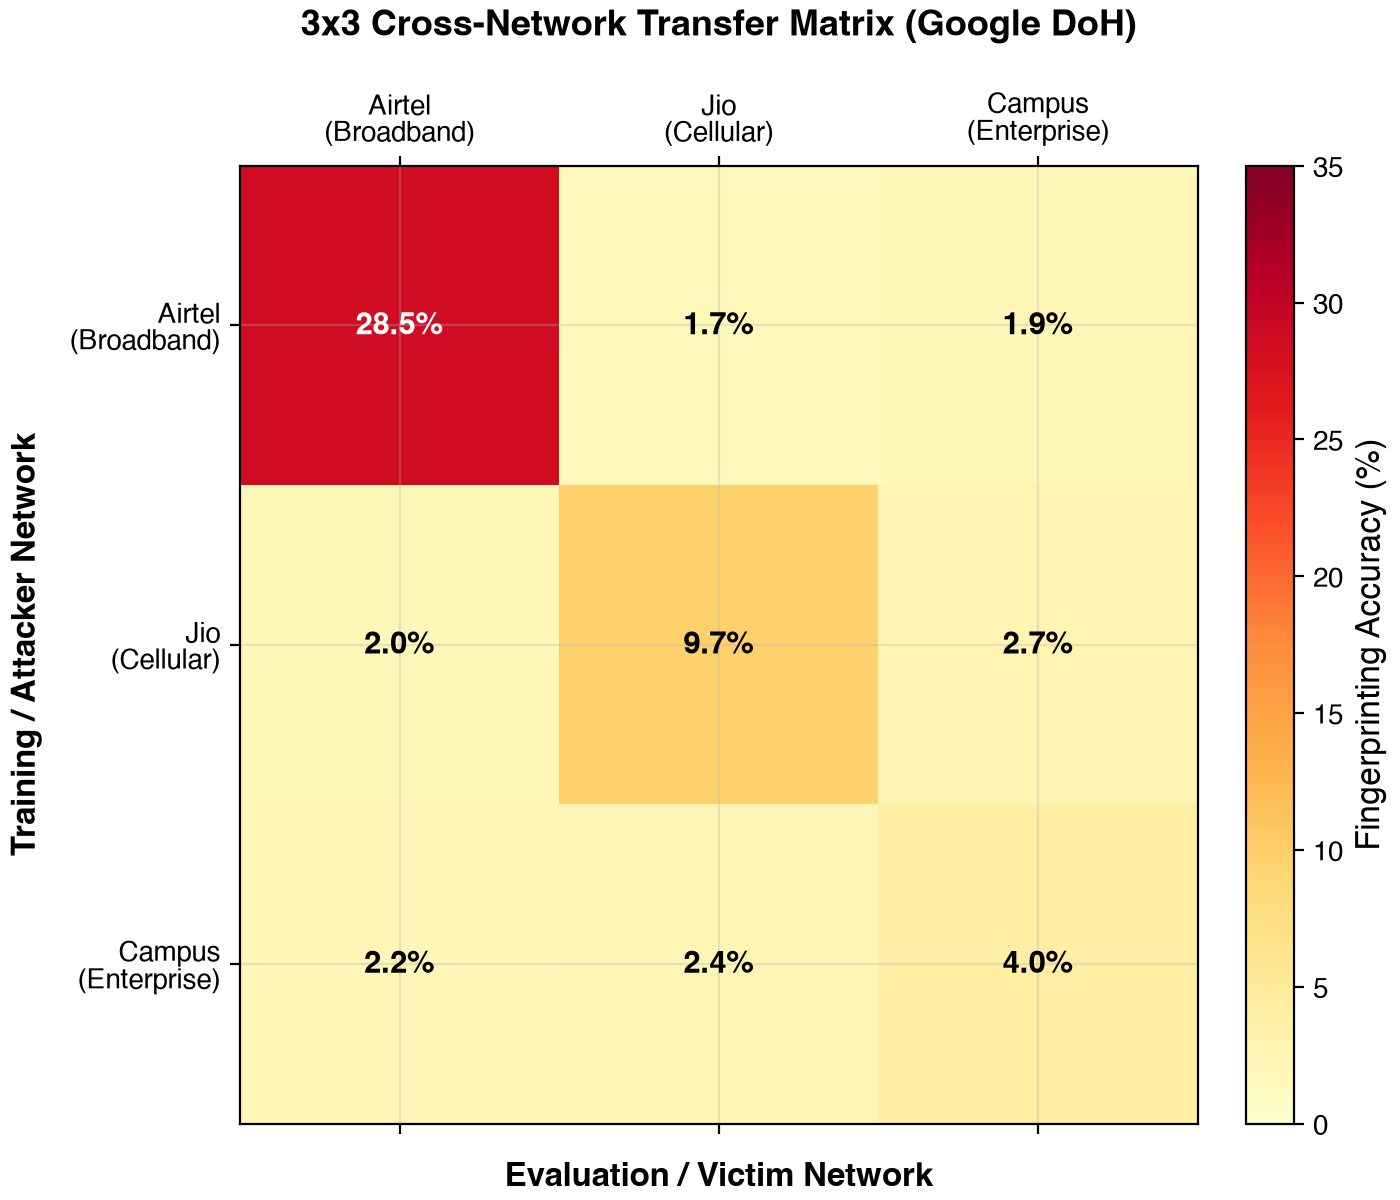
\includegraphics[width=0.48\textwidth]{figures/fig6_tri_network_transfer_matrix.png}
\caption{The $3 \times 3$ Cross-Network Transfer Matrix heatmap illustrating complete domain collapse along off-diagonal cross-network evaluations.}
\label{fig:transfer_matrix}
\end{figure}

The empirical results show \textbf{complete domain collapse}: an Airtel-trained classifier drops from 28.5\% within-network accuracy to 1.7\% on Jio and 1.9\% on Campus Wi-Fi (both below the 2.0\% chance baseline). 

To identify the root cause of this failure, we computed two-sample Kolmogorov-Smirnov (KS) statistics between empirical CDFs $F_1$ and $F_2$ across network pairs:
\begin{equation}
D = \sup_{u} |F_1(u) - F_2(u)|.
\label{eq:ks}
\end{equation}
We discovered massive distribution shifts ($p < 10^{-15}$): (1)~\texttt{up\_max} exhibits $D = 0.994$ due to carrier encapsulation offsets; (2)~\texttt{pkt\_00} exhibits $D = 0.837$, caused by direction inversion when campus proxy clients receive initial HTTP CONNECT acknowledgements ($-137$\,B) rather than issuing upstream handshakes ($+698$\,B); and (3)~\texttt{t\_first\_down} exhibits $D = 0.727$ due to cellular radio scheduling delays.

\subsection{Tri-Network Pooled Co-Training}
To evaluate whether an attacker with multiple capture points can overcome this limitation, we evaluated a multi-vantage adversary pooling training data across Airtel, Jio, and Campus networks (Table~\ref{tab:tri_network_pooled}).

\begin{table}[t]
\centering
\caption{Tri-Network Pooled Co-Training Evaluation (Google DoH Global, 50 shared domains, chance baseline $= 0.020$).}
\label{tab:tri_network_pooled}
\footnotesize
\setlength{\tabcolsep}{2.5pt}
\begin{tabular}{lrrrr}
\toprule
\textbf{Test Vantage}            & \textbf{Train}      & \textbf{Test}      & \textbf{Acc.}     & \textbf{95\% CI} \\
\midrule
\textbf{Held-Out Airtel}         & 1,120               & 100                & \textbf{0.180}    & [0.113, 0.250] \\
\textbf{Held-Out Jio}            & 1,120               & 100                & \textbf{0.140}    & [0.080, 0.207] \\
\textbf{Held-Out Campus}         & 1,120               & 90                 & \textbf{0.037}    & [0.004, 0.078] \\
\midrule
\textbf{Composite Tri-Network}   & \textbf{1,120}      & \textbf{290}       & \textbf{0.122}    & [0.087, 0.162] \\
\midrule
\textbf{Mean Across All 6 Slices}& --                  & --                 & \textbf{0.207}    & -- \\
\bottomrule
\end{tabular}
\end{table}

Multi-network pooling successfully restores classification capability, achieving \textbf{12.2\%} composite accuracy on Google Global (6.1$\times$ chance) and a mean of \textbf{20.7\%} across all six multi-network slices. While models cannot generalize to unseen networks zero-shot, an adversary pooling multi-carrier observations builds resilient models that learn carrier-invariant decision boundaries.

% =========================================================================
\section{Countermeasure Evaluation}
\label{sec:defenses}
% =========================================================================

We simulated four client- and resolver-side defense mechanisms on the representative AdGuard DoH Global slice (baseline accuracy 20.4\%):
\begin{enumerate}
    \item \textbf{Constant-Rate Block Padding:} Packet frame lengths are padded to the next integer block multiple:
    \begin{equation}
    s'_i = \lceil s_i / B \rceil \cdot B, \quad B \in \{64, 128\}\text{ bytes}.
    \label{eq:padding}
    \end{equation}
    \item \textbf{Random Padding:} Uniform noise $r \in [0, 128]$ bytes added to each frame: $s'_i = s_i + r$.
    \item \textbf{Delay Jitter:} Independent uniform latency jitter $j \in [0, 50]$\,ms or $j \in [0, 200]$\,ms injected into packet inter-arrival times.
\end{enumerate}

\begin{table}[t]
\centering
\caption{Simulated Defense Mechanisms on AdGuard DoH Global.}
\label{tab:defenses}
\footnotesize
\setlength{\tabcolsep}{2.5pt}
\begin{tabular}{llr}
\toprule
\textbf{Defense Mechanism} & \textbf{Configuration} & \textbf{Accuracy} \\
\midrule
\textbf{No Defense (Baseline)}   & None                       & \textbf{0.204} \\
\textbf{Constant Block Padding}  & Block Size $B = 64$\,B     & \textbf{0.141} ($-31\%$) \\
\textbf{Constant Block Padding}  & Block Size $B = 128$\,B    & \textbf{0.138} ($-32\%$) \\
\textbf{Random Padding}          & Uniform $r \in [0, 128]$\,B& \textbf{0.212} (No effect) \\
\textbf{Latency Jitter}          & $j \in [0, 50]$\,ms        & \textbf{0.201} (No effect) \\
\textbf{Latency Jitter}          & $j \in [0, 200]$\,ms       & \textbf{0.218} (No effect) \\
\bottomrule
\end{tabular}
\end{table}

As shown in Table~\ref{tab:defenses}, \textbf{constant-rate block padding reduces fingerprintability by $\approx 32\%$} (dropping accuracy from 20.4\% down to 13.8\%). Coarsening frame sizes into discrete blocks collapses fine-grained answer record variations. 

Conversely, \textbf{random padding and latency jitter provide zero protection}. Random noise simply expands aggregate flow distributions without masking relative order, while timing jitter does not alter volumetric features. Because tree classifiers rely primarily on cumulative volume and packet length extremes, temporal perturbations do not degrade classification performance.

% =========================================================================
\section{Related Work}
\label{sec:related}
% =========================================================================

Website fingerprinting (WF) has been extensively explored in Tor and encrypted VPN tunnels~\cite{herrmann2009website,sirinam2018deep,wang2017walkie}. In Tor WF, deep learning models achieve $>95\%$ accuracy on multi-megabyte page downloads spanning thousands of cells~\cite{sirinam2018deep,rimmer2018automated}. 

In encrypted DNS, Siby et al.~\cite{siby2020encrypted} and Bushart et al.~\cite{bushart2020padding} demonstrated that DoH and DoT traffic leak domain identities under laboratory conditions. Houser et al.~\cite{houser2019investigation} analyzed packet length features in DoT, while Hounsel et al.~\cite{hounsel2020comparing} compared DoH performance against DoT. However, these works focused primarily on HTTP/2 DoH on wired testbeds. Our research advances the state of the art by providing the first rigorous head-to-head empirical evaluation of production DoH/3 vs. DoH across multi-carrier mobile and institutional networks, uncovering real-world transport outages and cross-network transfer limits.

% =========================================================================
\newpage
\section{Conclusion}
\label{sec:conclusion}
% =========================================================================

In this paper, we presented a comprehensive empirical privacy evaluation of modern encrypted DNS across 31,200 real-world queries. We demonstrated that DoH/3 provides substantial privacy protection over DoH for three out of four resolvers, but identified that resolver implementation practices (e.g., Google Public DNS) can negate these protocol benefits. Crucially, we discovered that DoH/3 is currently unusable in production mobile cellular and institutional campus environments due to ubiquitous middlebox filtering of UDP port~443. We showed that cross-network fingerprinting models fail completely due to environmental distribution shifts, but multi-vantage pooling recovers adversarial accuracy. Finally, our findings establish that deterministic block padding is an effective, necessary countermeasure that must be standardized and deployed across resolvers to achieve genuine end-to-end DNS privacy.

\balance
\bibliographystyle{IEEEtran}
\bibliography{references}

\end{document}
